\subsection{Rectification}\label{subsec:rectification}

The rectification of two images is a process that finds two homographies $H_1$ and $H_2$ such that the two
homographied images have horizontal epipolar lines (or alternatively that the pixels of one image are all found at the
same $y$-level in the other image).

The first step of the algorithm is to run SIFT and match corresponding pairs of points.
ORSA (or RANSAC) is used to remove outliers (exactly as in the previous section) and find the fundamental matrix $F$.

The fundamental equation of epipolar geometry related how two corresponding points in two images must relate,
where $P_1$ and $P_2$ are the image coordinates of the two corresponding points (in homogeneous coordinates) and
$F$ is the fundamental matrix.
\begin{equation}\label{eq:fundamentalequationepipolargeometry}
    P_2^t F P_1=0
\end{equation}
In particular, equation~\eqref{eq:fundamentalequationepipolargeometry} states that if we know where a point is within
an image, the corresponding point in the other image will lie on a line.

If the images are rectified,
\[F=[e_1]_{\times}=\left[
\begin{array}{c c c}
    0 & 0 & 0\\
    0 & 0 & -1\\
    0 & 1 & 0
\end{array}\right]\]

This means that finding two homographies $H_R$ and $H_L$ such that:
\[F= H_R^t [e_1]_{\times} H_L\]
Is enough to rectify the two images since, by equation~\eqref{eq:fundamentalequationepipolargeometry}:
\[(H_R P_2)^t [e_1]_{\times} (H_L P_1) =0\]

The idea of the authors of~\citep{rectification} is to find rotations $R_R$ and $R_L$ that will rectify the images.
Rotating the camera with a rotation matrix $R$ is equivalent to the following homography $H$ (with $K$ the intrinsics
of the camera).
\[H=K R K^{-1}\]
Note that $K$ is not known in advance: $f$ is found at the same time as $R_R$ and $R_L$, and the principal point is
assumed to be at the center of both images.

Thus, the authors want to find $R_R$, $R_L$ and $f$ such that (note that $K^t [e_1]_{\times} K=f^2[e_1]_{\times})$:
\begin{align*}
    E(P_1,P_2,R_R,R_L,f)&=(K R_R K^{-1} P_2)[e_1]_{\times} (K R_L K^{-1} P_2)=P_2^t K^{-t} R_R^t K^t [e_1]_{\times} K R_L K^{-1} P_2\\
    &=P_2^t K^{-t} R_R^t f^2[e_1]_{\times} R_L K^{-1} P_2=0
\end{align*}

This can be reparametrized with $s=(\theta_{Ry},\theta_{Rz},\theta_{Lx},\theta_{Ly},\theta_{Lz},g)$ such that:
\[R_R=R_z(\theta_{Rz})R_y(\theta_{Ry})\hspace*{2em}R_L=R_z(\theta_{Lz})R_y(\theta_{Ly})R_x(\theta_{Lx})
\hspace*{2em} f=3^g (w+h)\]

Instead of minimizing the above error (which has no geometric interpretation but arises from algebra only), they
minimize the Sampson error:
\begin{equation}\label{eq:errorrectification}
    E_s(P_1,P_2)^2=E^t(JJ^t)^{-1}E
\end{equation}
Where $J$ is the jacobian of $E$ (in particular, computing $J$ requires the computation of
$\frac{\partial F}{\partial \theta_{Ry}},\frac{\partial F}{\partial \theta_{Rz}},\ldots$).

Using the continuous optimization algorithm of Levenberg-Marquardt, it is possible to find the best values for
$s=(\theta_{Ry},\theta_{Rz},\theta_{Lx},\theta_{Ly},\theta_{Lz},g)$ that minimize the sum of $E_s(P_1,P_2)^2$ for all
pairs of inlier points (\textit{QR.5}).

Figure~\ref{fig:rectification_base_images} shows two images of the same scene that we will rectify using the online
IPOL demo~\citep{rectification}.

\begin{figure}[ht]
    \centering
    \captionsetup{justification=centering}
    \begin{minipage}{.5\textwidth}
        \centering
    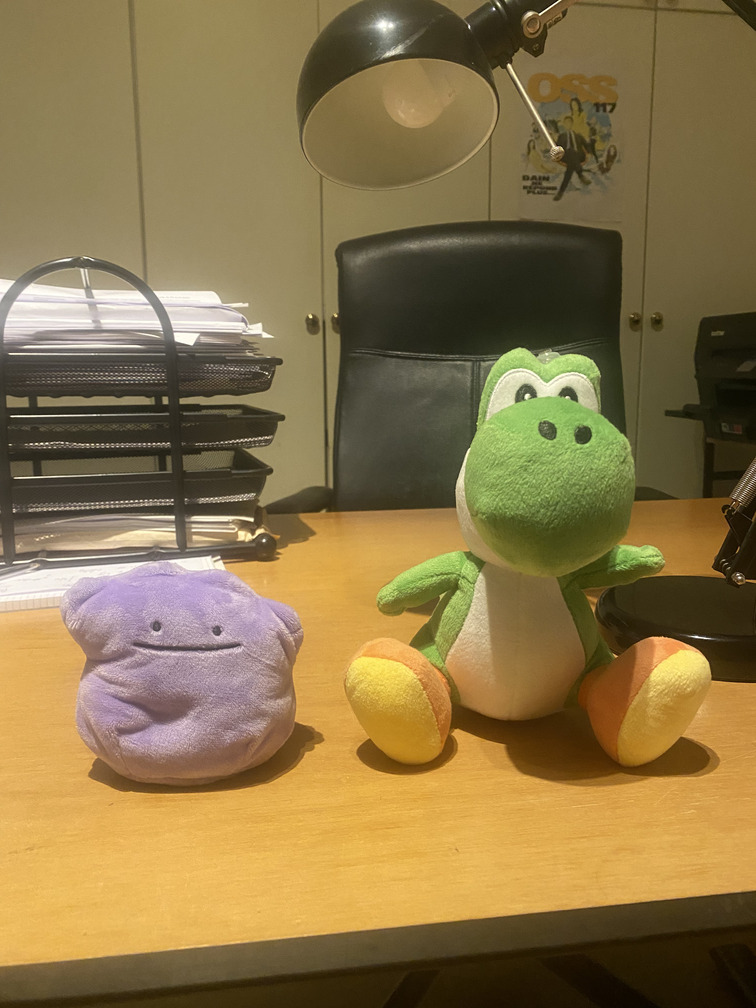
\includegraphics[width=0.6\textwidth]{assets/rectification/img_left}
    \end{minipage}%
    \hfill
    \begin{minipage}{.5\textwidth}
        \centering
    
\includegraphics[width=0.6\textwidth]{assets/rectification/img_right}
    \end{minipage}
    \caption{The two original images.}
    \label{fig:rectification_base_images}
\end{figure}

The rectified pair is given in figure~\ref{fig:rectified_images} (\textit{QR.1}, a \texttt{gif} version is provided
alongside this report).

\begin{figure}[ht]
    \centering
    \captionsetup{justification=centering}
    \begin{minipage}{.5\textwidth}
        \centering
    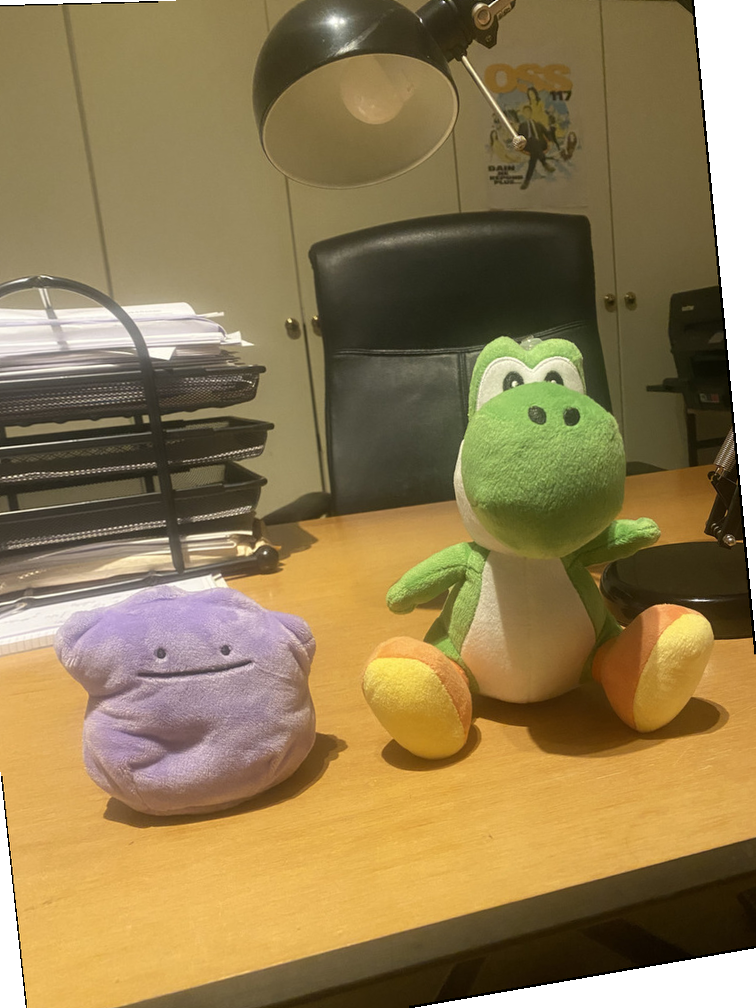
\includegraphics[width=0.6\textwidth]{assets/rectification/img_left_rect}
    \end{minipage}%
    \hfill
    \begin{minipage}{.5\textwidth}
        \centering
    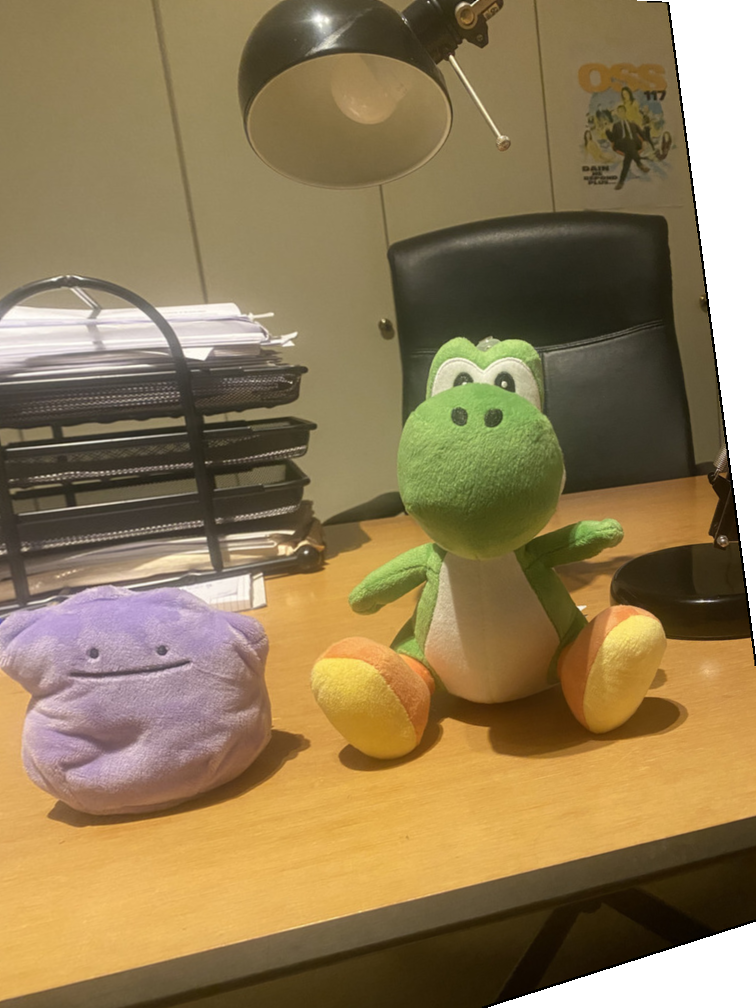
\includegraphics[width=0.6\textwidth]{assets/rectification/img_right_rect}
    \end{minipage}
    \caption{The two rectified images.}
    \label{fig:rectified_images}
\end{figure}

As mentioned before, the tool finds two homographies and applies them to the input images to find the rectified pair.
We give hereunder the homography for the right image.
\[H_R=\left[
\begin{array}{c c c}
    1.156 & 0.157 & -150.34\\
    0.0374 & 1.0078 & -26.91\\
    0.00035 & 0.0000349 & 0.81749
\end{array}\right]\]
We can verify that this homography indeed corresponds to the rectification of the right image by applying
it (\textit{QR.2}):
\begin{figure}[ht]
    \centering
    \captionsetup{justification=centering}
    \begin{minipage}{.5\textwidth}
        \centering
    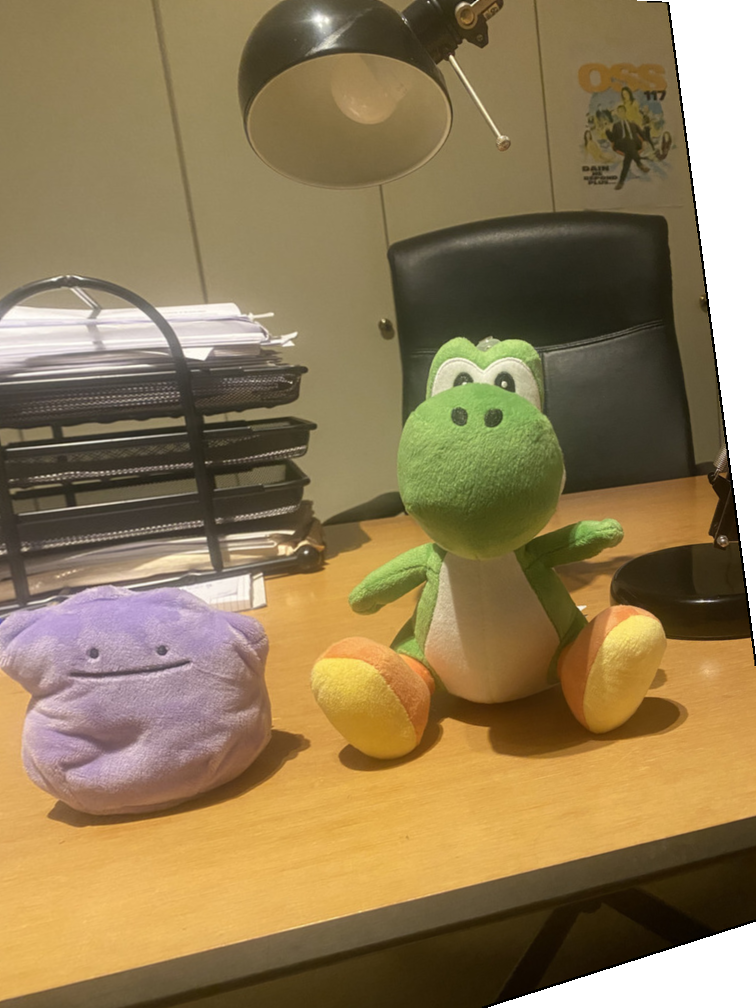
\includegraphics[width=0.6\textwidth]{assets/rectification/img_right_rect}
    \end{minipage}%
    \hfill
    \begin{minipage}{.5\textwidth}
        \centering
    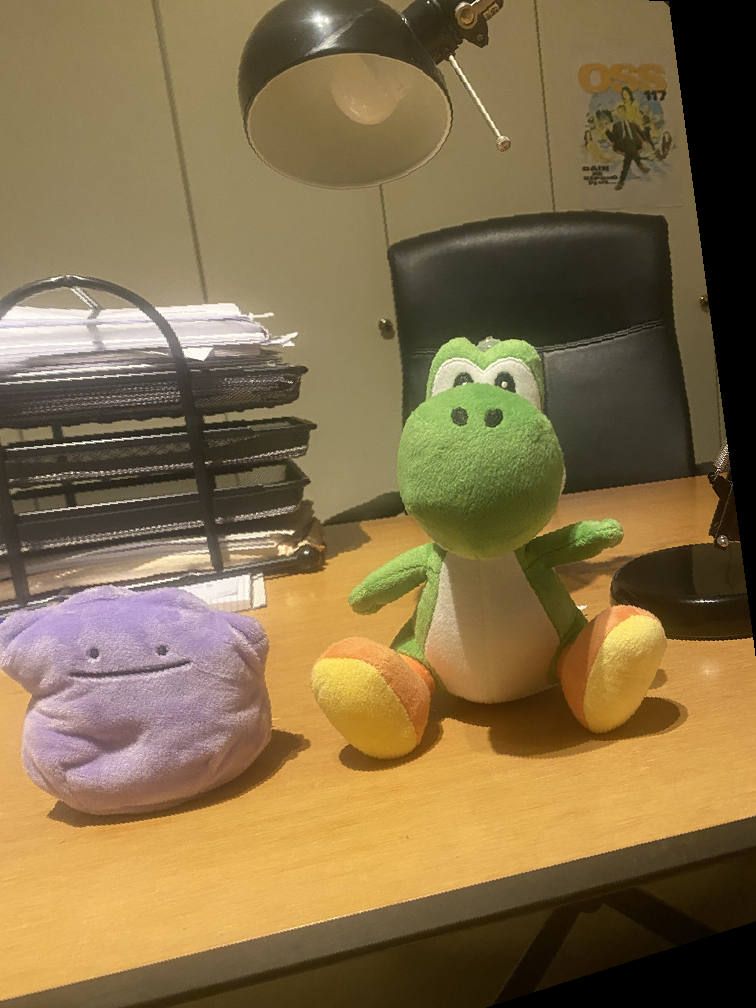
\includegraphics[width=0.6\textwidth]{assets/rectification/homographied_right_img}
    \end{minipage}
    \caption{The right output image (left) and the right input image homographied by $H_R$ (right).}
    \label{fig:righthomographiedimage}
\end{figure}

We will draw the epipolar line corresponding to the right armpit of Yoshi in the left image.
The right armpit of Yoshi lies at the point $(459,577)$, which means that $P_1=\left[\begin{array}{c c c}
                   459 & 577 &1\end{array}\right]^t$.
The online tool estimated $F$ for us.

\[F=\left[
\begin{array}{c c c}
    -1.41539e-08 & 2.82758e-07 & -1.6399e-05\\
    -8.97881e-08 & 7.82147e-09 & -0.0009103\\
    -3.28468e-05 & 0.000803705 & 0.0285408
\end{array}
\right]\]

Since we know $P_1$ and $F$, we can compute the epipolar line.
If $FP_1=\left[\begin{array}{c c c}
                   a & b & c
\end{array}\right]^t $, then the equation of the epipolar line is
(by equation~\eqref{eq:fundamentalequationepipolargeometry}):
\[y=\frac{-ax-c}{b}\]
In figure~\ref{fig:yoshi_epipolar}, we show this epipolar line, and we can observe that indeed, the right armpit of Yoshi
lies on the line (\textit{QR.3}).

\begin{figure}[ht]
    \centering
    \captionsetup{justification=centering}
    \begin{minipage}{.5\textwidth}
        \centering
    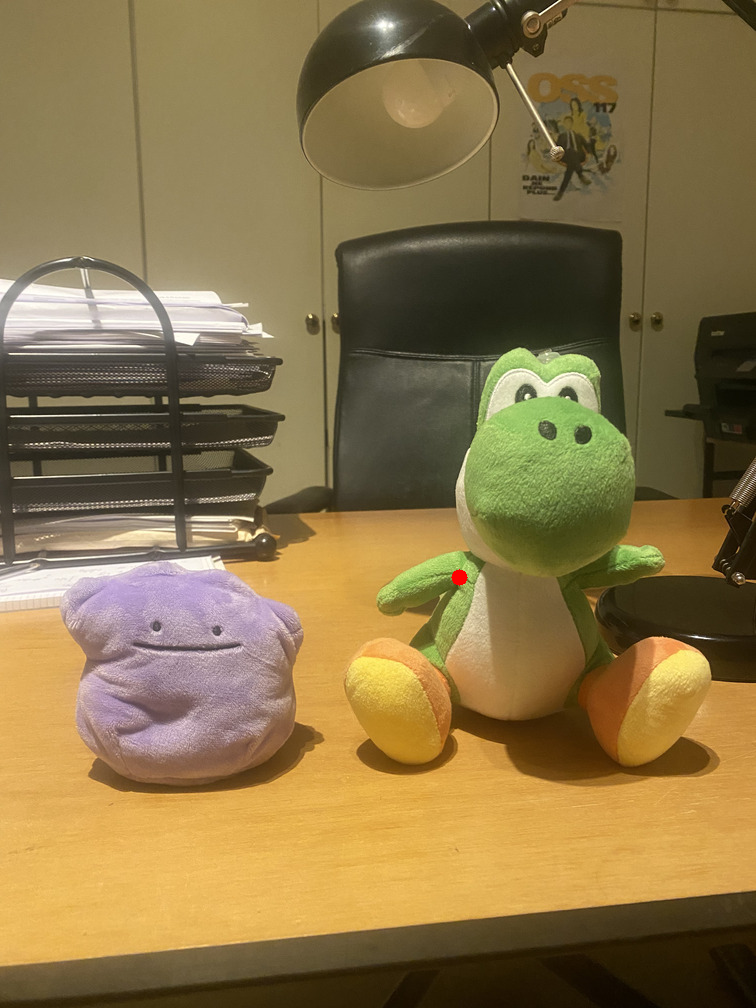
\includegraphics[width=0.7\textwidth]{assets/rectification/yoshi_epipolar_left}
    \end{minipage}%
    \hfill
    \begin{minipage}{.5\textwidth}
        \centering
    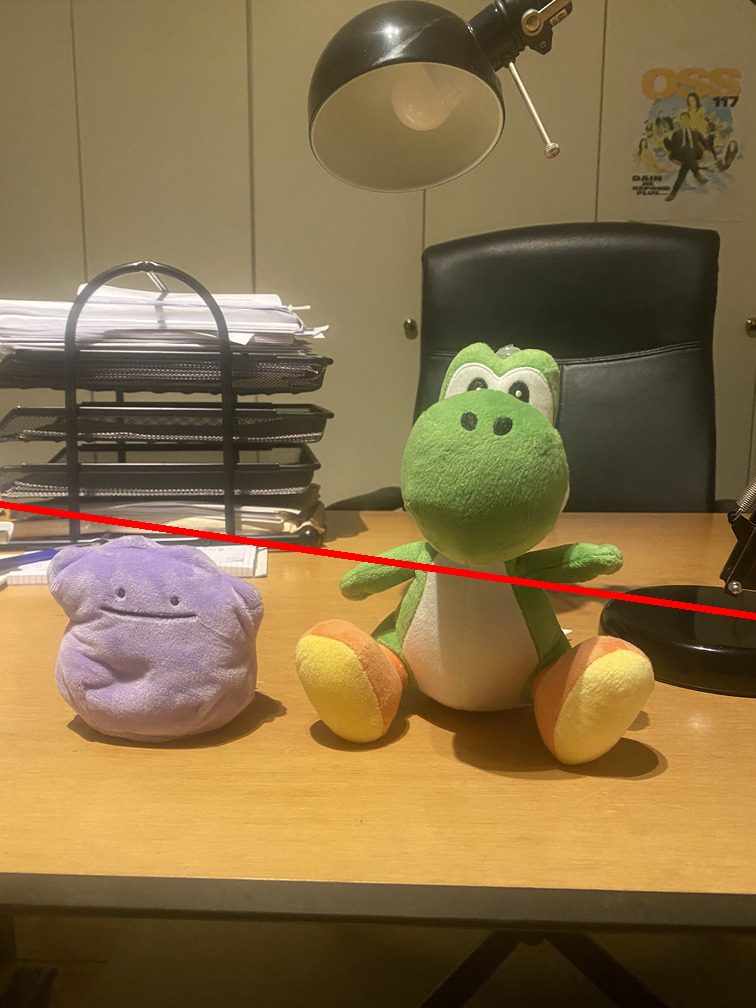
\includegraphics[width=0.7\textwidth]{assets/rectification/yoshi_epipolar_right}
    \end{minipage}
    \caption{The two original images but with the epipolar line (in the right image) corresponding to the point on the
    right armpit of Yoshi (in the left image).}
    \label{fig:yoshi_epipolar}
\end{figure}

The focal length was estimated by the online tool, and we are thus able to build the two intrinsics matrices (assuming
the principal point is in the center of the $756\times 1006$ pixels images).
Note that the $K_1$, $K_2$ matrices that the tool outputs are the intrinsics for the cameras of the homographied images.
\[K_L=\left[
\begin{array}{c c c}
    731.057 & 0 & 378\\
    0 & 731.057 & 504\\
    0 & 0 & 1
\end{array}\right]\hspace*{2em}
K_R=\left[
\begin{array}{c c c}
    731.057 & 0 & 378\\
    0 & 731.057 & 504\\
    0 & 0 & 1
\end{array}\right]\]

The essential matrix $E=RT_{[\times]}$ holds information about the translation and rotation between the two shots.
The fundamental matrix can be written as the following product (which thus holds both the intrinsics and
extrinsics)\footnote{There is a typo in the syllabus, it's written $F=K_R^t EK_L$ on page 31.}:
\begin{equation*}
    E=K_R^t FK_L
\end{equation*}
We would like to retrieve the rotation and translation information for the two shots.
Using Singular Value Decomposition (SVD), we can decompose $E$:
\[E=RT_{[\times]}=U\Sigma V^t\]
With all three matrices above, it is possible to retrive $R$ and $T_{[\times]}$ out of four different possibilities:
\begin{align*}
        T_{[\times]}&=U(\pm W)\Sigma U^t\\
        R&=U(\pm W)^{-1}V^t
\end{align*}

Where:
\[\pm W=\left[\begin{array}{c c c}
              0 & \pm 1 & 0\\
              \mp 1 & 0 & 0\\
              0 & 0 & 1
\end{array}\right]\]

We can apply this procedure on the two images of figure~\ref{fig:rectification_base_images}.
This gives four different possibities for $(R,t)$ with only one that is correct.
We extrinsics between the left and the right shot are (\textit{QR.4}):
\[t=\lambda\left[\begin{array}{c c c}
    0.572 & 0.0713 & -0.138
\end{array}\right]^t\hspace*{2em}R=\left[\begin{array}{c c c}
    0.987 & -0.0397 & 0.151 \\
    0.0392 & 0.999 & 0.00637 \\
    -0.151 & -0.000371 & 0.989
\end{array}\right]\]
We were able to isolate the correct pair $(R,t)$ because only one of the two possible $t$ had a positive $x$ component
and only one of the two possible $R$ did not make the camera look into the opposite direction (flipped the $z$ axis).

We can visualize these extrinsics using an online tool such as
\\\href{https://dugas.ch/transform_viewer/index.html}{https://dugas.ch/transform\_viewer/index.html}
(figure~\ref{fig:rect_twocameras}).

\begin{figure}[H]
    \centering
    \captionsetup{justification=centering}
    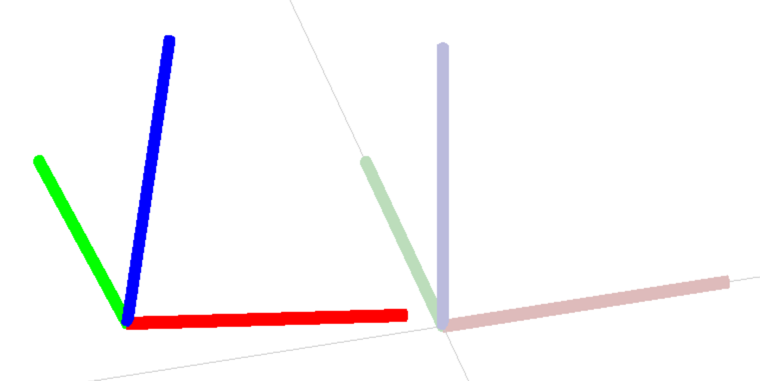
\includegraphics[width=0.4\textwidth]{assets/rectification/twocameras}
    \caption{The position in space of the two cameras according to the found extrinsics $R,t$.
    Note that the $x$-axis (red) is flipped and the $z$-axis (blue) is the depth axis.
    The dim origin represents the position of the left camera and the brighter one the right camera.}
    \label{fig:rect_twocameras}
\end{figure}

The issue is that the translation is only known up to scale.
To retrieve the size of the baseline, we can approximate the depth of some pixel and its disparity and then apply
the following equation to retrieve the baseline, where $Z$ is the depth (in $mm$), $B$ the baseline (in $mm$), $f$
the focal length (in $px$) and $d$ the disparity (in $px$):

\begin{equation}\label{eq:disparitydepth}
    Z=B\frac{f}{d}\Longleftrightarrow B=\frac{dZ}{f}
\end{equation}

We will consider the upmost point of Yoshi's two eyes.
The top pixel of Yoshi's right eye (the one on the left from the camera's point of view) is located at $(512,372)$ and
left eye is located at $(552,370)$.
We have $\Delta x'=552-512=40$ and $\Delta y'=372-370=2$.

We have seen in the lecture that the image point $(x',y')$ has the coordinates $(X,Y,Z)$ is 3D space, where:
\[x'=p_x+\frac{f_x X}{Z}\hspace*{2em} y'=p_y+\frac{f_y Y}{Z}\]
Here, $f_x=f_y=f$.
Rearranging the terms,
\[X=\frac{Z(x'-p_x)}{f}\hspace*{2em} Y=\frac{Z(y'-p_y)}{f}\]
We have that the difference in $X$ and $Y$ coordinates of the two considered points is:
\[\Delta X=X_1-X_2=\frac{Z(x'_1-p_x)}{f}-\frac{Z(x'_2-p_x)}{f}=\frac{Z\Delta x'}{f}\hspace*{2em} \Delta Y=\frac{Z\Delta y'}{f}\]
Note that we want to find the depth $Z$.
The real-life distance between the top of the two eyes is of approximately $D=19.3mm$.
This distance is equal to ($\Delta Z=0$ since we have picked points at the same depth):
\[D=\sqrt{\Delta X^2+\Delta Y^2+\Delta Z^2}=\sqrt{\Delta X^2+\Delta Y^2}\]
Combining everything, we have:
\[D=\sqrt{\left(\frac{Z\Delta x'}{f}\right)^2+\left(\frac{Z\Delta y'}{f}\right)^2}=\frac{Z}{f}\sqrt{(\Delta x')^2+(\Delta y')^2}\]
Finally, rearranging the terms:
\[Z=\frac{Df}{\sqrt{(\Delta x')^2+(\Delta y')^2}}\]
Plugging in $f=731.057$ (found by the only tool), $\Delta x'=40$, $\Delta y'=2$ and $D=19.3$ (all found manually),
we obtain $Z=352.29mm$.

All that is left to compute to apply equation~\eqref{eq:disparitydepth} is to find the disparity of Yoshi's highest
right eye's point (we could have considered the left eye, it does not matter since both point have the same depth and
hence the same disparity).
In the right image, the pixel is located at $(463,372)$.
The disparity is $d=512-463=49$ pixels (and indeed, we can check that the disparity is 49 as well for the other eye,
justifying our choice of reference points: both eyes truly lie at roughly the same depth $Z$).

Applying the equation, we find $B=23.61mm$.
This distance seems reasonable (most of the difference in perspective came from the rotation).

To find the true translation $t_{mm}$, we can simply normalize $t$ and multiply it by the baseline.
\[t_{mm}=B\frac{t}{\left\|t\right\|}\]

Hence, the true values for $t$ (in $mm$) and $R$ are:
\[t_{mm}=\left[\begin{array}{c c c}
    22.78 & 2.839 & -5.497
\end{array}\right]^t\hspace*{2em}R=\left[\begin{array}{c c c}
    0.987 & -0.0397 & 0.151 \\
    0.0392 & 0.999 & 0.00637 \\
    -0.151 & -0.000371 & 0.989
\end{array}\right]\]